\documentclass{article}
\usepackage{tikz}
\usetikzlibrary{matrix}

\begin{document}

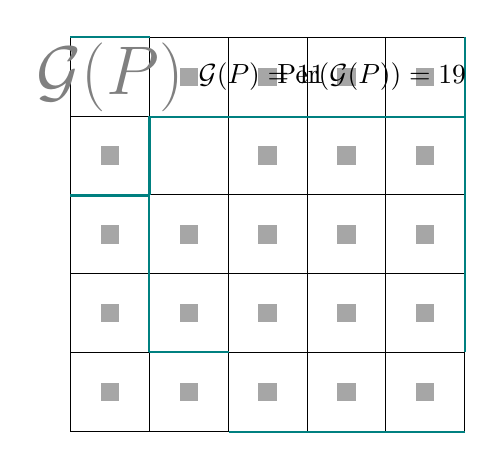
\begin{tikzpicture}[scale=0.5]
    \matrix (m) [matrix of nodes, nodes={minimum size=1cm, draw, anchor=center},
                 row sep=-\pgflinewidth, column sep=-\pgflinewidth,
                 nodes in empty cells] {
        & & & & \\
        & & & & \\
        & & & & \\
        & & & & \\
        & & & & \\
    };
    
    % Fill the cluster in gray
    \foreach \i/\j in {1/2, 1/3, 1/4, 1/5, 2/1, 2/3, 2/4, 2/5, 3/1, 3/2, 3/3, 3/4, 3/5, 4/1, 4/2, 4/3, 4/4, 4/5, 5/1, 5/2, 5/3, 5/4, 5/5} {
        \node[fill=gray!70] at (m-\i-\j) {};
    }
    
    % Draw the perimeter in teal
    \draw[teal, thick] (m-1-2.south west) -- (m-1-5.south east);
    \draw[teal, thick] (m-1-5.north east) -- (m-5-5.north east);
    \draw[teal, thick] (m-5-5.south east) -- (m-5-2.south east);
    \draw[teal, thick] (m-5-2.north east) -- (m-5-2.north west);
    \draw[teal, thick] (m-5-2.north west) -- (m-2-2.north west);
    \draw[teal, thick] (m-2-2.south west) -- (m-2-1.south west);
    \draw[teal, thick] (m-2-1.south west) -- (m-2-1.south east);
    \draw[teal, thick] (m-2-1.south east) -- (m-1-1.south east);
    \draw[teal, thick] (m-1-1.north east) -- (m-1-1.north west);
    \draw[teal, thick] (m-1-1.north west) -- (m-1-2.north west);
    
    \node at (m-1-1) {\textcolor{gray}{\Huge$\mathcal{G}(P)$}};
    \node at (m-1-1) [right=1cm] {$\abs{\mathcal{G}(P)} = 11$};
    \node at (m-1-1) [right=2cm] {$\mathrm{Per}(\mathcal{G}(P)) = 19$};
\end{tikzpicture}

\end{document}